\documentclass{beamer}

\usefonttheme{structurebold}

\usepackage[utf8]{inputenc}
\usepackage[T1]{fontenc}
\usepackage[portuguese]{babel} 



\title{Introdução ao \LaTeX}
\date{\today}
\author{Ricardo Peixoto Robaina \\ Techelinux Bagé}
\institute{Universidade Federal do Pampa}

\usetheme{unipampa}




\begin{document}
	
	\begin{frame}[noframenumbering]
		\titlepage
		\thispagestyle{empty}
	\end{frame}
	
	\begin{frame}{Sumário}
		\setbeamertemplate{section in toc}[sections numbered]
		\tableofcontents[hideallsubsections]
	\end{frame}

\section{Introdução}
\begin{frame}{Introdução}
	
	Sed ut perspiciatis unde omnis iste natus error sit voluptatem accusantium doloremque laudantium, totam rem aperiam, eaque ipsa quae ab illo inventore veritatis et quasi architecto beatae vitae dicta sunt explicabo. Nemo enim ipsam voluptatem quia voluptas sit aspernatur aut odit aut fugit, sed quia consequuntur magni dolores eos qui ratione voluptatem sequi nesciunt. 
	
	\begin{itemize}
		\item Blá
		\item Blá
		\item Blá
	\end{itemize}

\end{frame}


\section{Instalação}
\begin{frame}{Intalação}

	\begin{block}{TexLive (Baixa todos os pacotes)}
		\begin{itemize}
			\item sudo apt-get install texlive-full
			\\Baixa todos os pacotes  
		\end{itemize}
	\end{block}
	
	
	\begin{block}{MikTeX (Baixa os pacotes sob demanda)}
		\begin{itemize}
			\item https://miktex.org/howto/install-miktex-unx
			
			\item sudo apt-key adv --keyserver hkp://keyserver.ubuntu.com:80 --recv-keys D6BC243565B2087BC3F897C9277A7293F59E4889
			
			\item echo "deb http://miktex.org/download/ubuntu bionic universe" | sudo tee /etc/apt/sources.list.d/miktex.list
			
			\item sudo apt-get update
			
			\item sudo apt-get install miktex
		\end{itemize}
	\end{block}
	

\end{frame}


\begin{frame}{Atualização MikTeX}

	\begin{figure}[!htb]
		\centering
		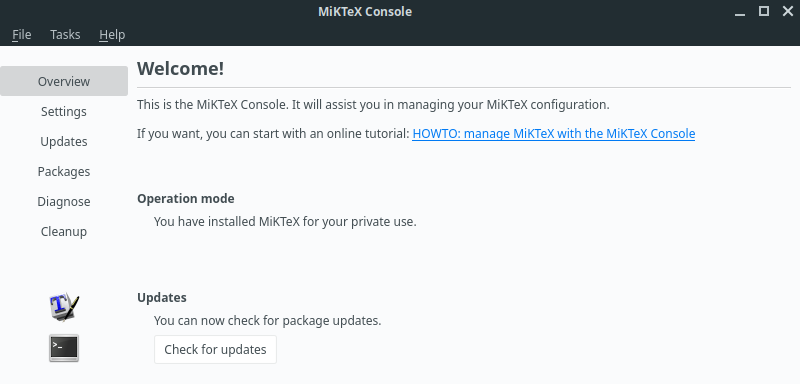
\includegraphics[scale=.38]{miktex.png}
	\end{figure}

\end{frame}

\begin{frame}{Intalação}

	\begin{block}{TexStudio (IDE)}
		\begin{itemize}
			\item sudo apt-get install texstudio
		\end{itemize}
	\end{block}
	
	

	\begin{block}{Resumindo}
		\begin{itemize}
			\item sudo apt-get install texlive-full texstudio 
		\end{itemize}
	\end{block}

\end{frame}


\section{Estrutura dos Documentos}

\begin{frame}{Estrutura}

	\begin{figure}[!htb]
		\centering
		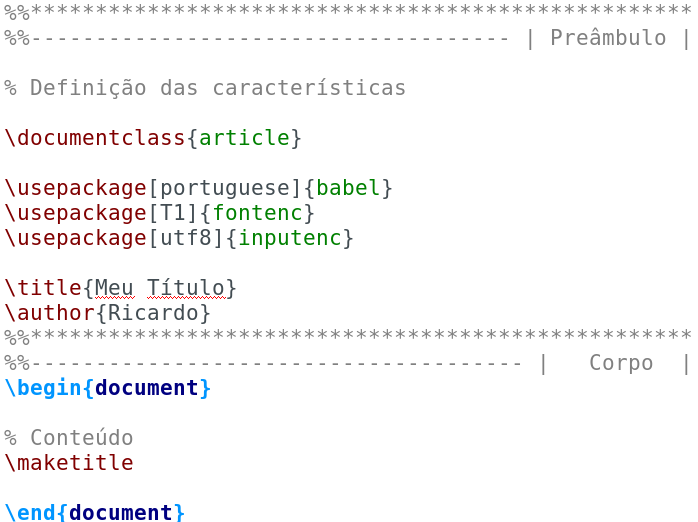
\includegraphics[scale=.4]{estrutura.png}
	\end{figure}

\end{frame}


\begin{frame}{Compilação}
	
	\begin{itemize}
		\item criar o arquivo.tex
		\item pdflatex arquivo.tex
	\end{itemize}

\end{frame}




\section{Criando um Texto}
\begin{frame}{Criando um Texto}

	\begin{itemize}
		\item $\backslash$documentclass\{article\}
		\item $\backslash$documentclass\{book\}
		\item $\backslash$documentclass\{report\}
		\item $\backslash$documentclass\{...\}
	\end{itemize}
	

\end{frame}


\section{Criando um Slide}

	\begin{frame}{Criando um Slide}
	
	\begin{itemize}
		\item $\backslash$documentclass\{beamer\}
	\end{itemize}

\end{frame}

\section{Referências}
	
\begin{frame}{Referências}
	
	
			\begin{itemize}
				\item https://www.latex-project.org/ \\
				
\includegraphics[width=0.5\textwidth]{latex-project-logo.png}
				
				
				\item LaTeX: A Document Preparation System (Leslie Lamport) \\
				
\includegraphics[scale=0.2]{livro.png}
			\end{itemize}

	
	
\end{frame}

\begin{frame}{Introdução ao \LaTeX}
	
		\newline
		\begin{center}
			{\Huge  \textbf{Obrigado!} \\}
		\end{center}
		
		{\normalsize 
			\begin{itemize}
				\item ricardorobaina11@gmail.com 
				\item https://github.com/robainaricardo/tchelinux \\ \newline   
			\end{itemize}	
		}
		\maketitle
	
\end{frame}



\end{document}